\documentclass[UTF8,zihao=-4]{ctexart}
\usepackage[a4paper,margin=2.5cm]{geometry}
\usepackage{amsmath, amssymb, amsthm}
\usepackage{bm}
\usepackage{hyperref}
\usepackage{graphicx}
\usepackage{caption}
\usepackage{listings}
\usepackage{xcolor}
\usepackage{float}
\usepackage{placeins}
\graphicspath{{figures/}}

% Code style
\lstdefinestyle{code}{
  basicstyle=\ttfamily\small,
  numbers=left,
  numberstyle=\tiny,
  numbersep=8pt,
  keywordstyle=\color{blue},
  commentstyle=\color{teal!70!black},
  stringstyle=\color{orange!70!black},
  showstringspaces=false,
  breaklines=true,
  frame=single,
  framerule=0.3pt,
  rulecolor=\color{black!15}
}
\lstset{style=code}

\title{深度网络训练教程}
\author{}
\date{\today}

\begin{document}
\maketitle

\section{反向传播算法}
反向传播利用链式法则高效计算标量损失 $\mathcal{L}$ 对所有网络参数的梯度。设 $L$ 层全连接网络满足 $\mathbf{h}^{(\ell)} = \phi^{(\ell)}\bigl(\mathbf{a}^{(\ell)}\bigr)$,$\mathbf{a}^{(\ell)} = \mathbf{W}^{(\ell)} \mathbf{h}^{(\ell-1)} + \mathbf{b}^{(\ell)}$。损失对预激活的梯度向后传播:
\begin{equation}
  \boldsymbol{\delta}^{(\ell)} = \bigl(\mathbf{W}^{(\ell+1)}\bigr)^{\top} \boldsymbol{\delta}^{(\ell+1)} \odot \phi'^{(\ell)}\bigl(\mathbf{a}^{(\ell)}\bigr),
\end{equation}
其中 $\odot$ 表示逐元素乘,末层梯度 $\boldsymbol{\delta}^{(L)} = \nabla_{\mathbf{h}^{(L)}} \mathcal{L}$。参数梯度为
\begin{align}
  \nabla_{\mathbf{W}^{(\ell)}} \mathcal{L} &= \boldsymbol{\delta}^{(\ell)} \bigl(\mathbf{h}^{(\ell-1)}\bigr)^{\top}, \\
  \nabla_{\mathbf{b}^{(\ell)}} \mathcal{L} &= \boldsymbol{\delta}^{(\ell)}.
\end{align}
图~\ref{fig:backprop_graph_cn} 展示了前向与反向的信息流。

向量-雅可比积的观点可推广至任意计算图:对中间变量 $\mathbf{z}$,其局部雅可比矩阵为 $\mathbf{J} = \partial \mathbf{z} / \partial \boldsymbol{\theta}$,反向传播通过 $\mathbf{J}^{\top} \nabla_{\mathbf{z}} \mathcal{L}$ 获得 $\nabla_{\boldsymbol{\theta}} \mathcal{L}$,无需显式构造雅可比矩阵。

\begin{lstlisting}[language=Python, caption={密集网络的小批量反向传播示例。}]
def backward_pass(weights, activations, preacts, grads_out, loss_grad):
    deltas = [None] * len(weights)
    deltas[-1] = loss_grad
    for l in reversed(range(len(weights) - 1)):
        W_next = weights[l + 1]
        delta_next = deltas[l + 1]
        deltas[l] = (W_next.T @ delta_next) * activations[l] * (1 - activations[l])
    grad_W = [delta @ a.T for delta, a in zip(deltas, preacts)]
    grad_b = [delta.sum(axis=1, keepdims=True) for delta in deltas]
    return grad_W, grad_b
\end{lstlisting}

\begin{figure}[H]
  \centering
  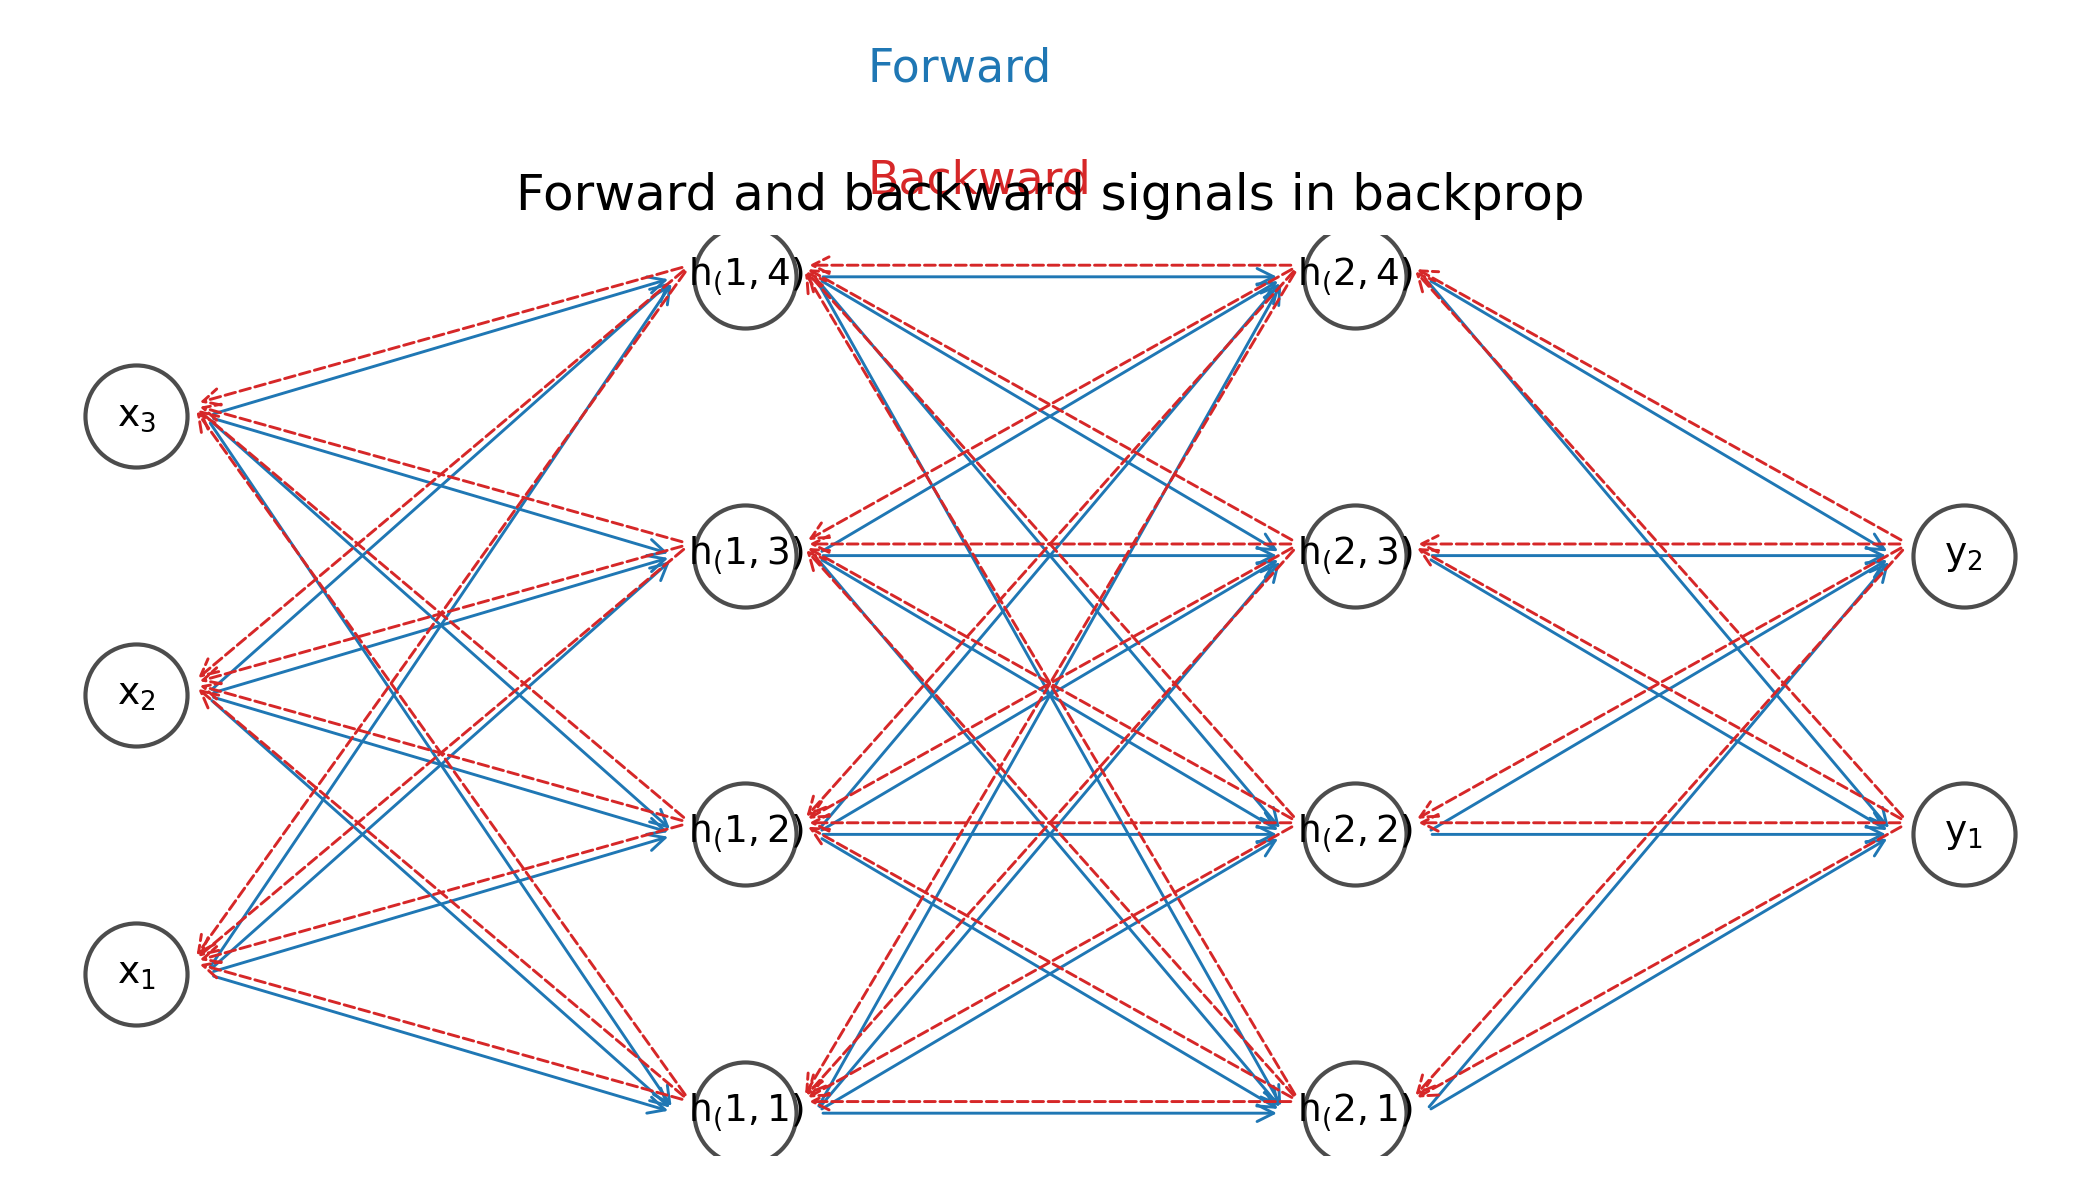
\includegraphics[width=0.8\linewidth]{backprop_computational_graph.png}
  \caption{层状网络的前向(实线)与反向(虚线)传播路径。}
  \label{fig:backprop_graph_cn}
\end{figure}
\FloatBarrier

\section{梯度下降方法}
在得到梯度 $\nabla_{\boldsymbol{\theta}} \mathcal{L}$ 后,通过迭代更新参数以最小化损失。图~\ref{fig:optimization_trajectories_cn} 比较了多种优化路径。

\subsection{随机梯度下降(SGD)}
SGD 使用来自小批量 $\mathcal{B}_t$ 的噪声梯度:
\begin{equation}
  \boldsymbol{\theta}_{t+1} = \boldsymbol{\theta}_t - \eta_t \nabla_{\boldsymbol{\theta}} \mathcal{L}(\boldsymbol{\theta}_t; \mathcal{B}_t).
\end{equation}
学习率 $\eta_t$ 可保持常数或随训练调整。采样噪声有助于逃离陡峭局部极值,但可能降低收敛速度。

\subsection{动量法}
动量法累积速度向量 $\mathbf{v}_t$:
\begin{align}
  \mathbf{v}_{t+1} &= \mu \mathbf{v}_t - \eta_t \nabla_{\boldsymbol{\theta}} \mathcal{L}(\boldsymbol{\theta}_t), \\
  \boldsymbol{\theta}_{t+1} &= \boldsymbol{\theta}_t + \mathbf{v}_{t+1},
\end{align}
其中 $\mu \in [0,1)$ 为动量系数,可沿稳定下降方向加速,并抑制峡谷中的震荡。

\subsection{Nesterov 加速梯度(NAG)}
Nesterov 动量先做预测再修正:
\begin{align}
  \tilde{\boldsymbol{\theta}}_t &= \boldsymbol{\theta}_t + \mu \mathbf{v}_t, \\
  \mathbf{v}_{t+1} &= \mu \mathbf{v}_t - \eta_t \nabla_{\boldsymbol{\theta}} \mathcal{L}(\tilde{\boldsymbol{\theta}}_t), \\
  \boldsymbol{\theta}_{t+1} &= \boldsymbol{\theta}_t + \mathbf{v}_{t+1}.
\end{align}
在预估位置计算梯度可获得更强的理论收敛保证,实践中也往往更快。

\begin{figure}[H]
  \centering
  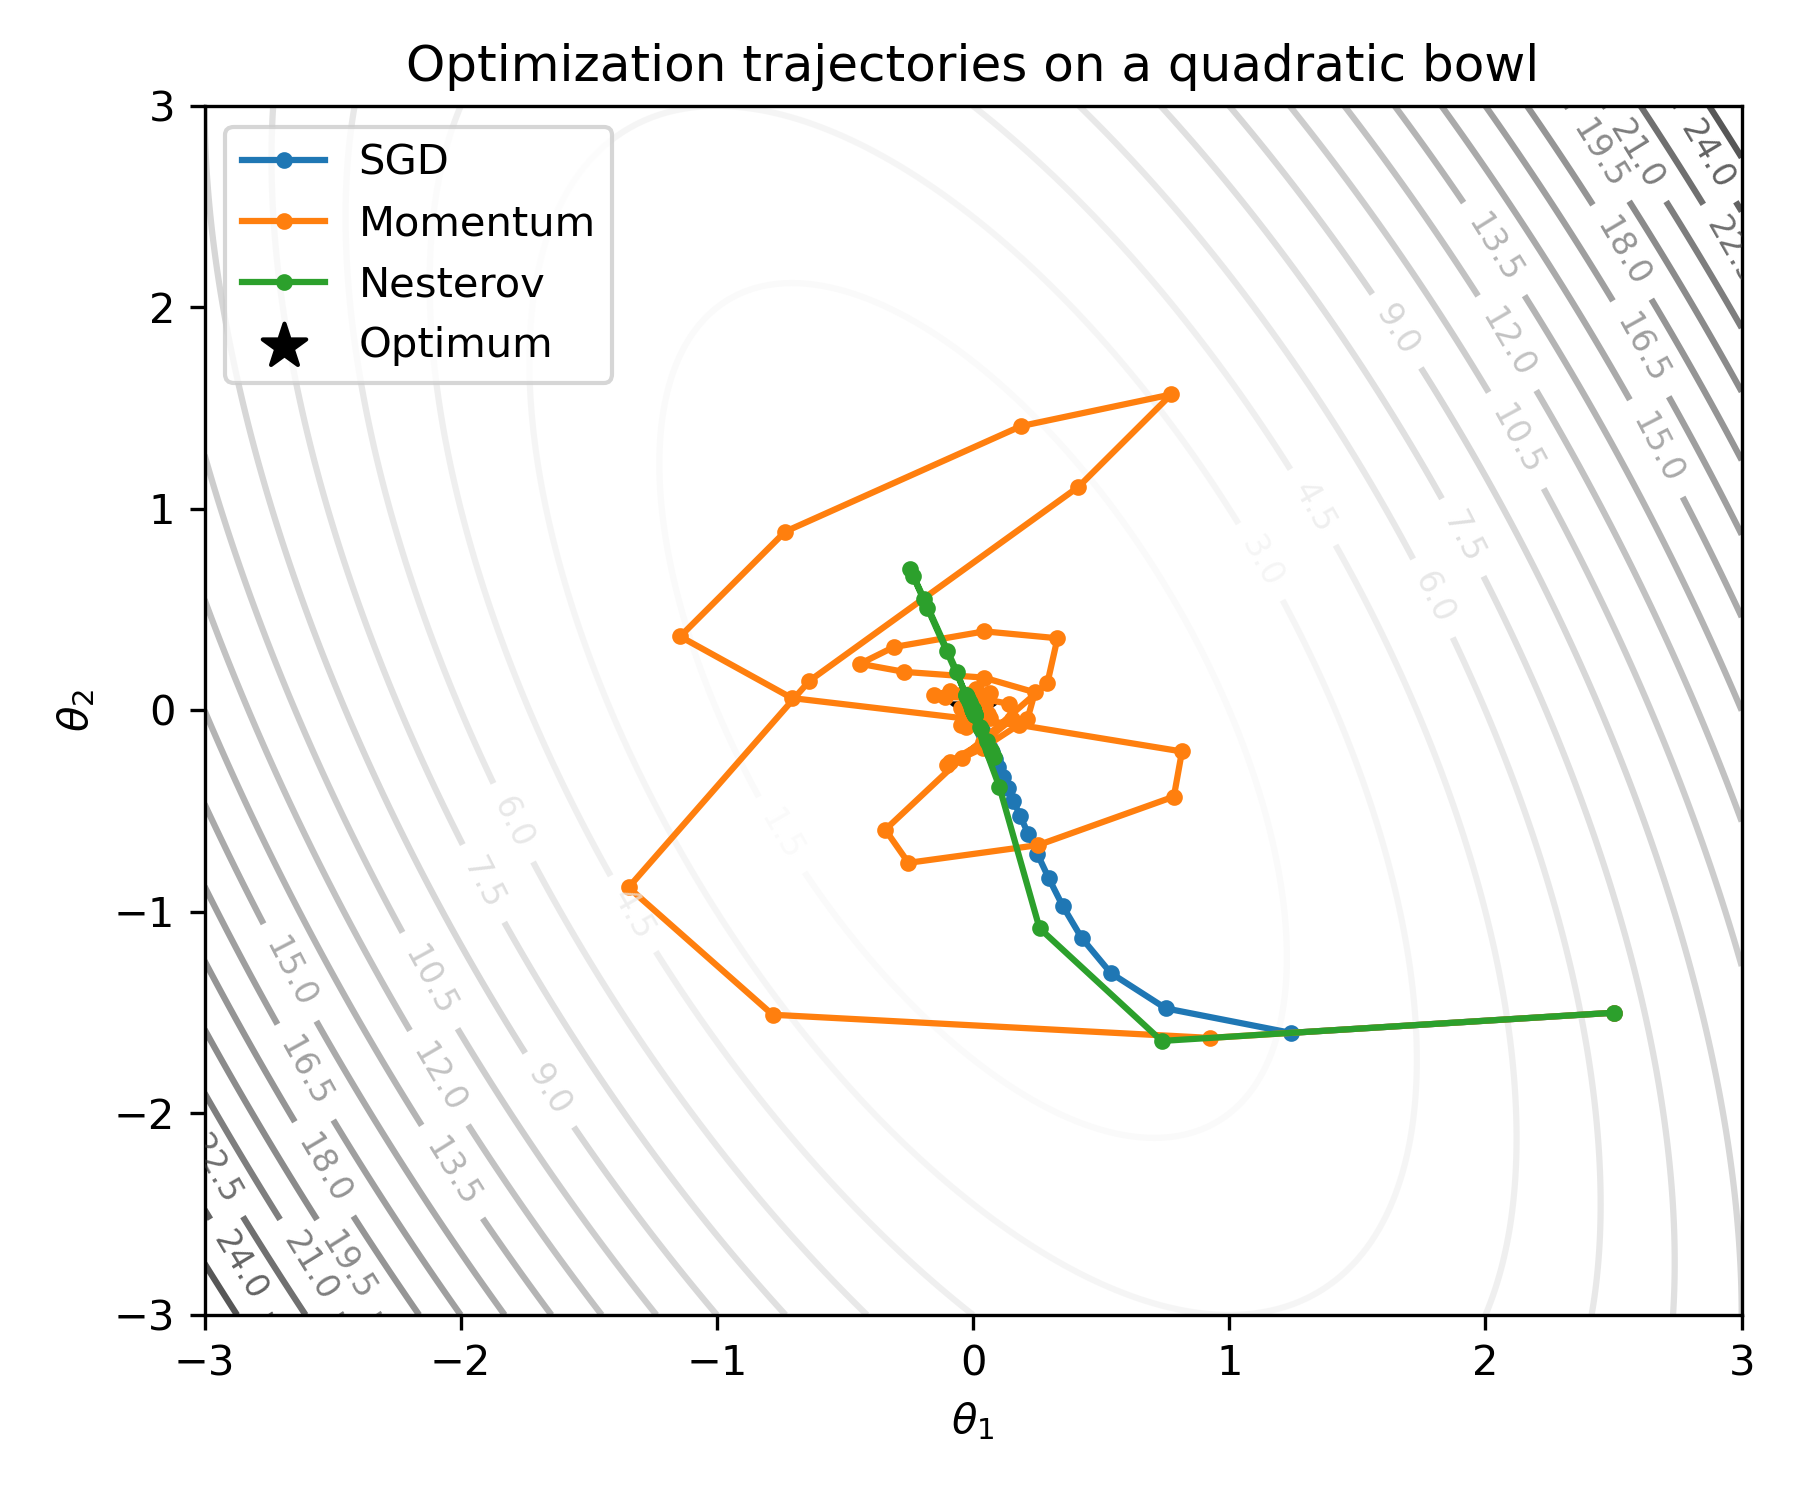
\includegraphics[width=0.8\linewidth]{optimization_trajectories.png}
  \caption{曲面二次函数上不同优化方法的参数轨迹。}
  \label{fig:optimization_trajectories_cn}
\end{figure}
\FloatBarrier

\section{学习率调度}
合理的学习率调度兼顾快速下降与稳定收敛,常见策略包括:

\begin{itemize}
  \item \textbf{阶梯衰减:} 每隔 $k$ 个 epoch 将学习率乘以 $\gamma<1$,即 $\eta_t = \eta_0 \gamma^{\lfloor t/k \rfloor}$。
  \item \textbf{指数衰减:} 按 $\eta_t = \eta_0 \exp(-\lambda t)$ 连续下降。
  \item \textbf{余弦退火:} 在 $\eta_{\min}$ 与 $\eta_{\max}$ 间按余弦函数震荡,可结合周期性重启。
  \item \textbf{预热(Warmup):} 在前 $T_w$ 步线性升高学习率,再切换到主调度。
\end{itemize}

图~\ref{fig:lr_schedules_cn} 展示了多种调度及其预热阶段。即使使用 Adam、RMSprop 等自适应优化器,显式调度仍能带来收益。

\begin{figure}[H]
  \centering
  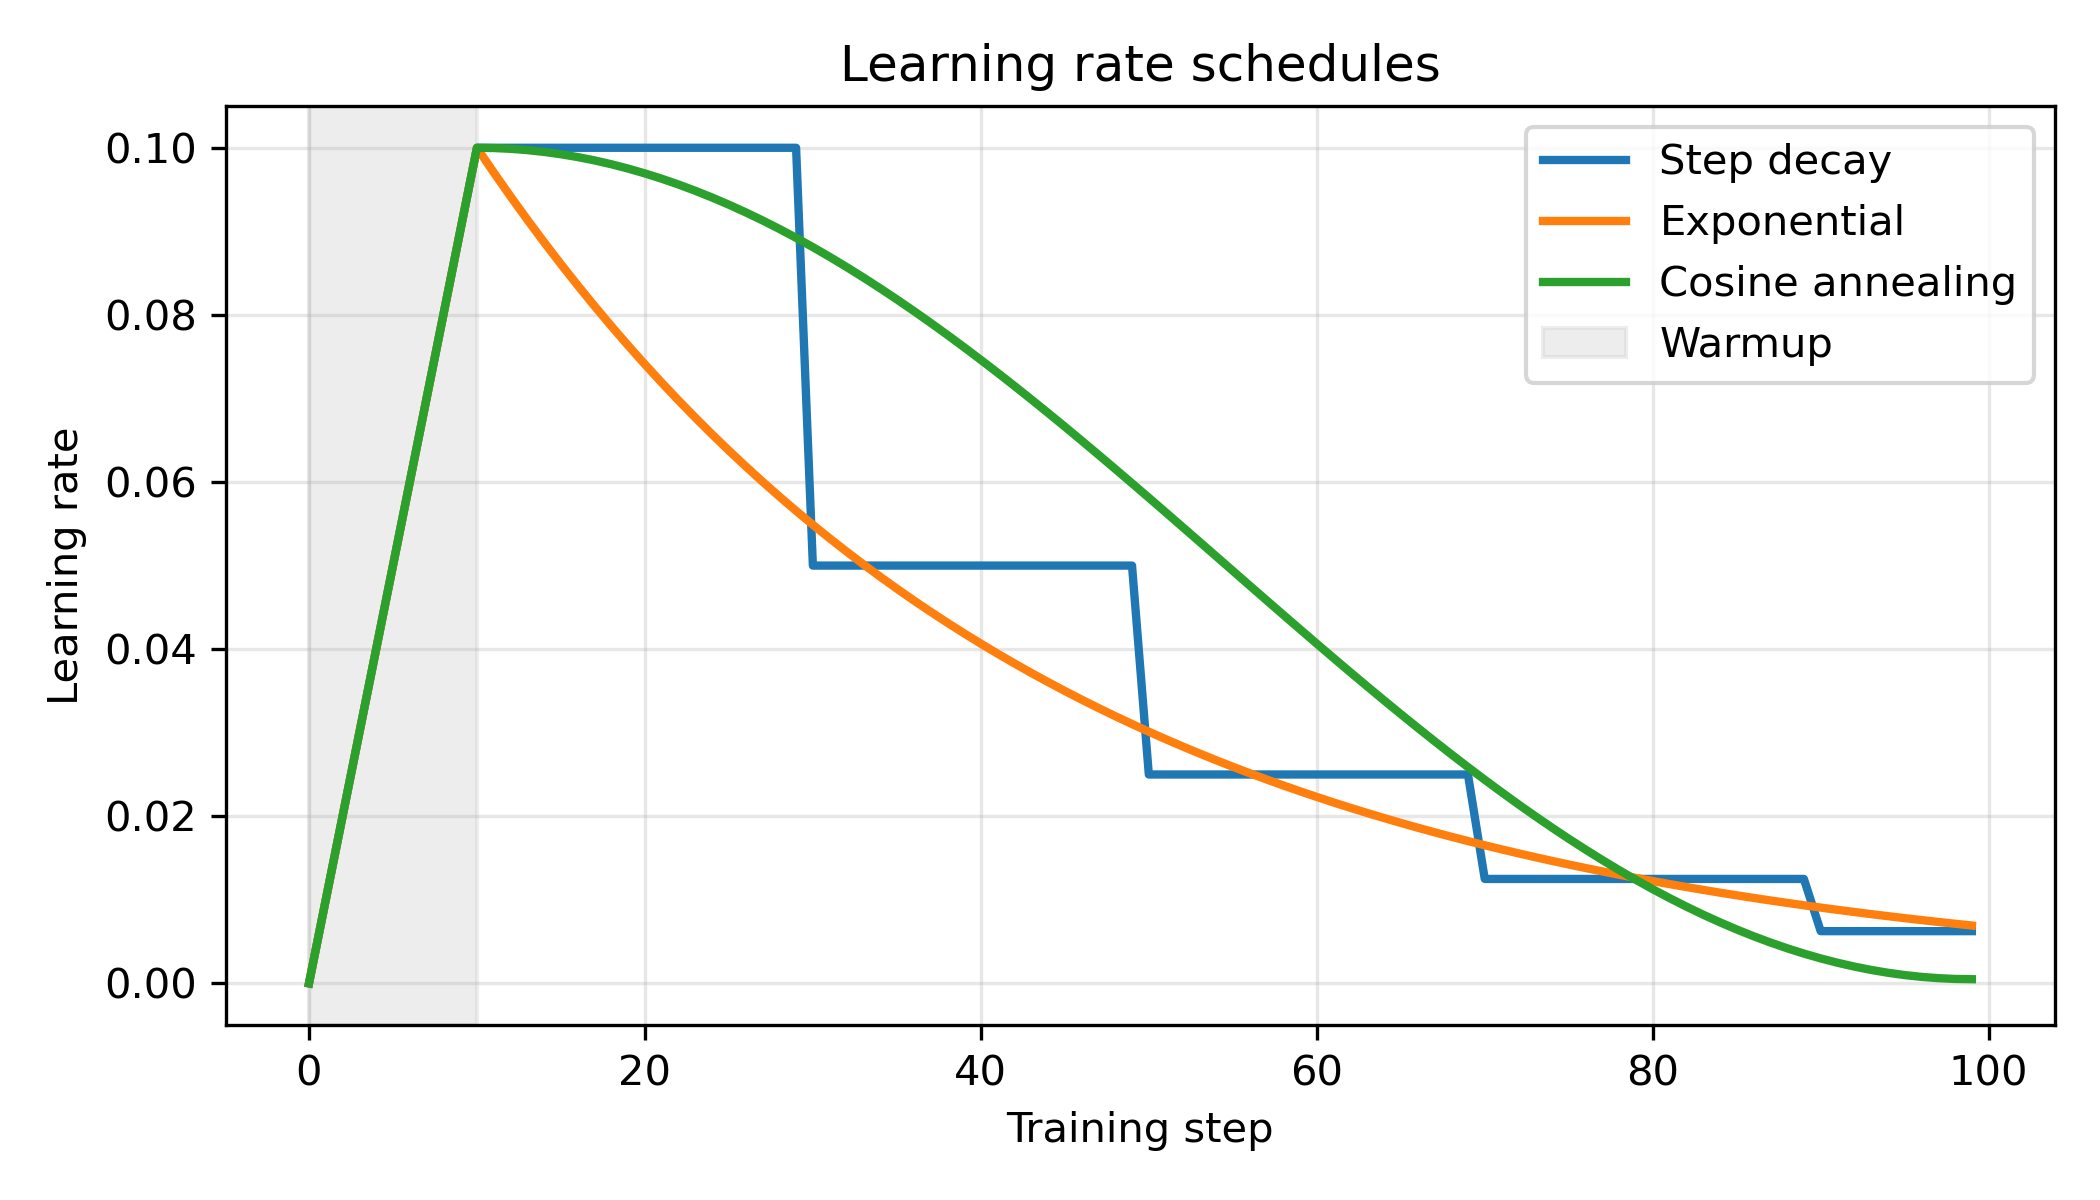
\includegraphics[width=0.8\linewidth]{learning_rate_schedules.png}
  \caption{带预热的学习率调度示例。}
  \label{fig:lr_schedules_cn}
\end{figure}
\FloatBarrier

\section{过拟合与正则化}
过拟合指模型在训练集上表现优异却无法泛化。图~\ref{fig:regularization_effects_cn} 显示了多种正则化手段缩小泛化差距的效果。

\subsection{权重惩罚}
L2 正则化在损失中加入 $\lambda \|\boldsymbol{\theta}\|_2^2$,对应权重衰减;L1 正则化加入 $\lambda \|\boldsymbol{\theta}\|_1$,可诱导稀疏。两者对应的梯度为
\begin{align}
  \nabla_{\boldsymbol{\theta}} (\mathcal{L} + \lambda \|\boldsymbol{\theta}\|_2^2) &= \nabla_{\boldsymbol{\theta}} \mathcal{L} + 2\lambda \boldsymbol{\theta}, \\
  \nabla_{\boldsymbol{\theta}} (\mathcal{L} + \lambda \|\boldsymbol{\theta}\|_1) &= \nabla_{\boldsymbol{\theta}} \mathcal{L} + \lambda\, \mathrm{sign}(\boldsymbol{\theta}).
\end{align}

\subsection{Dropout}
Dropout 在训练中以保留概率 $p$ 随机屏蔽激活,采样掩码 $\mathbf{m} \sim \mathrm{Bernoulli}(p)$,得到 $\tilde{\mathbf{h}} = \mathbf{m} \odot \mathbf{h}$。推理阶段按 $p$ 缩放激活。该方法抑制特征共适应,近似集成多个子网络。

\subsection{数据增强}
数据增强通过裁剪、翻转、颜色扰动等保持标签不变的变换扩展训练分布,引入归纳偏置并降低方差。

\subsection{Batch Normalization}
BatchNorm 使用小批量统计量对激活进行归一化:
\begin{align}
  \hat{\mathbf{h}} &= \frac{\mathbf{h} - \boldsymbol{\mu}_\mathcal{B}}{\sqrt{\boldsymbol{\sigma}_\mathcal{B}^2 + \epsilon}}, \\
  \mathbf{y} &= \boldsymbol{\gamma} \odot \hat{\mathbf{h}} + \boldsymbol{\beta}.
\end{align}
该方法能稳定激活分布,使得更大学习率成为可能,同时批量噪声也提供正则效果。

\begin{figure}[H]
  \centering
  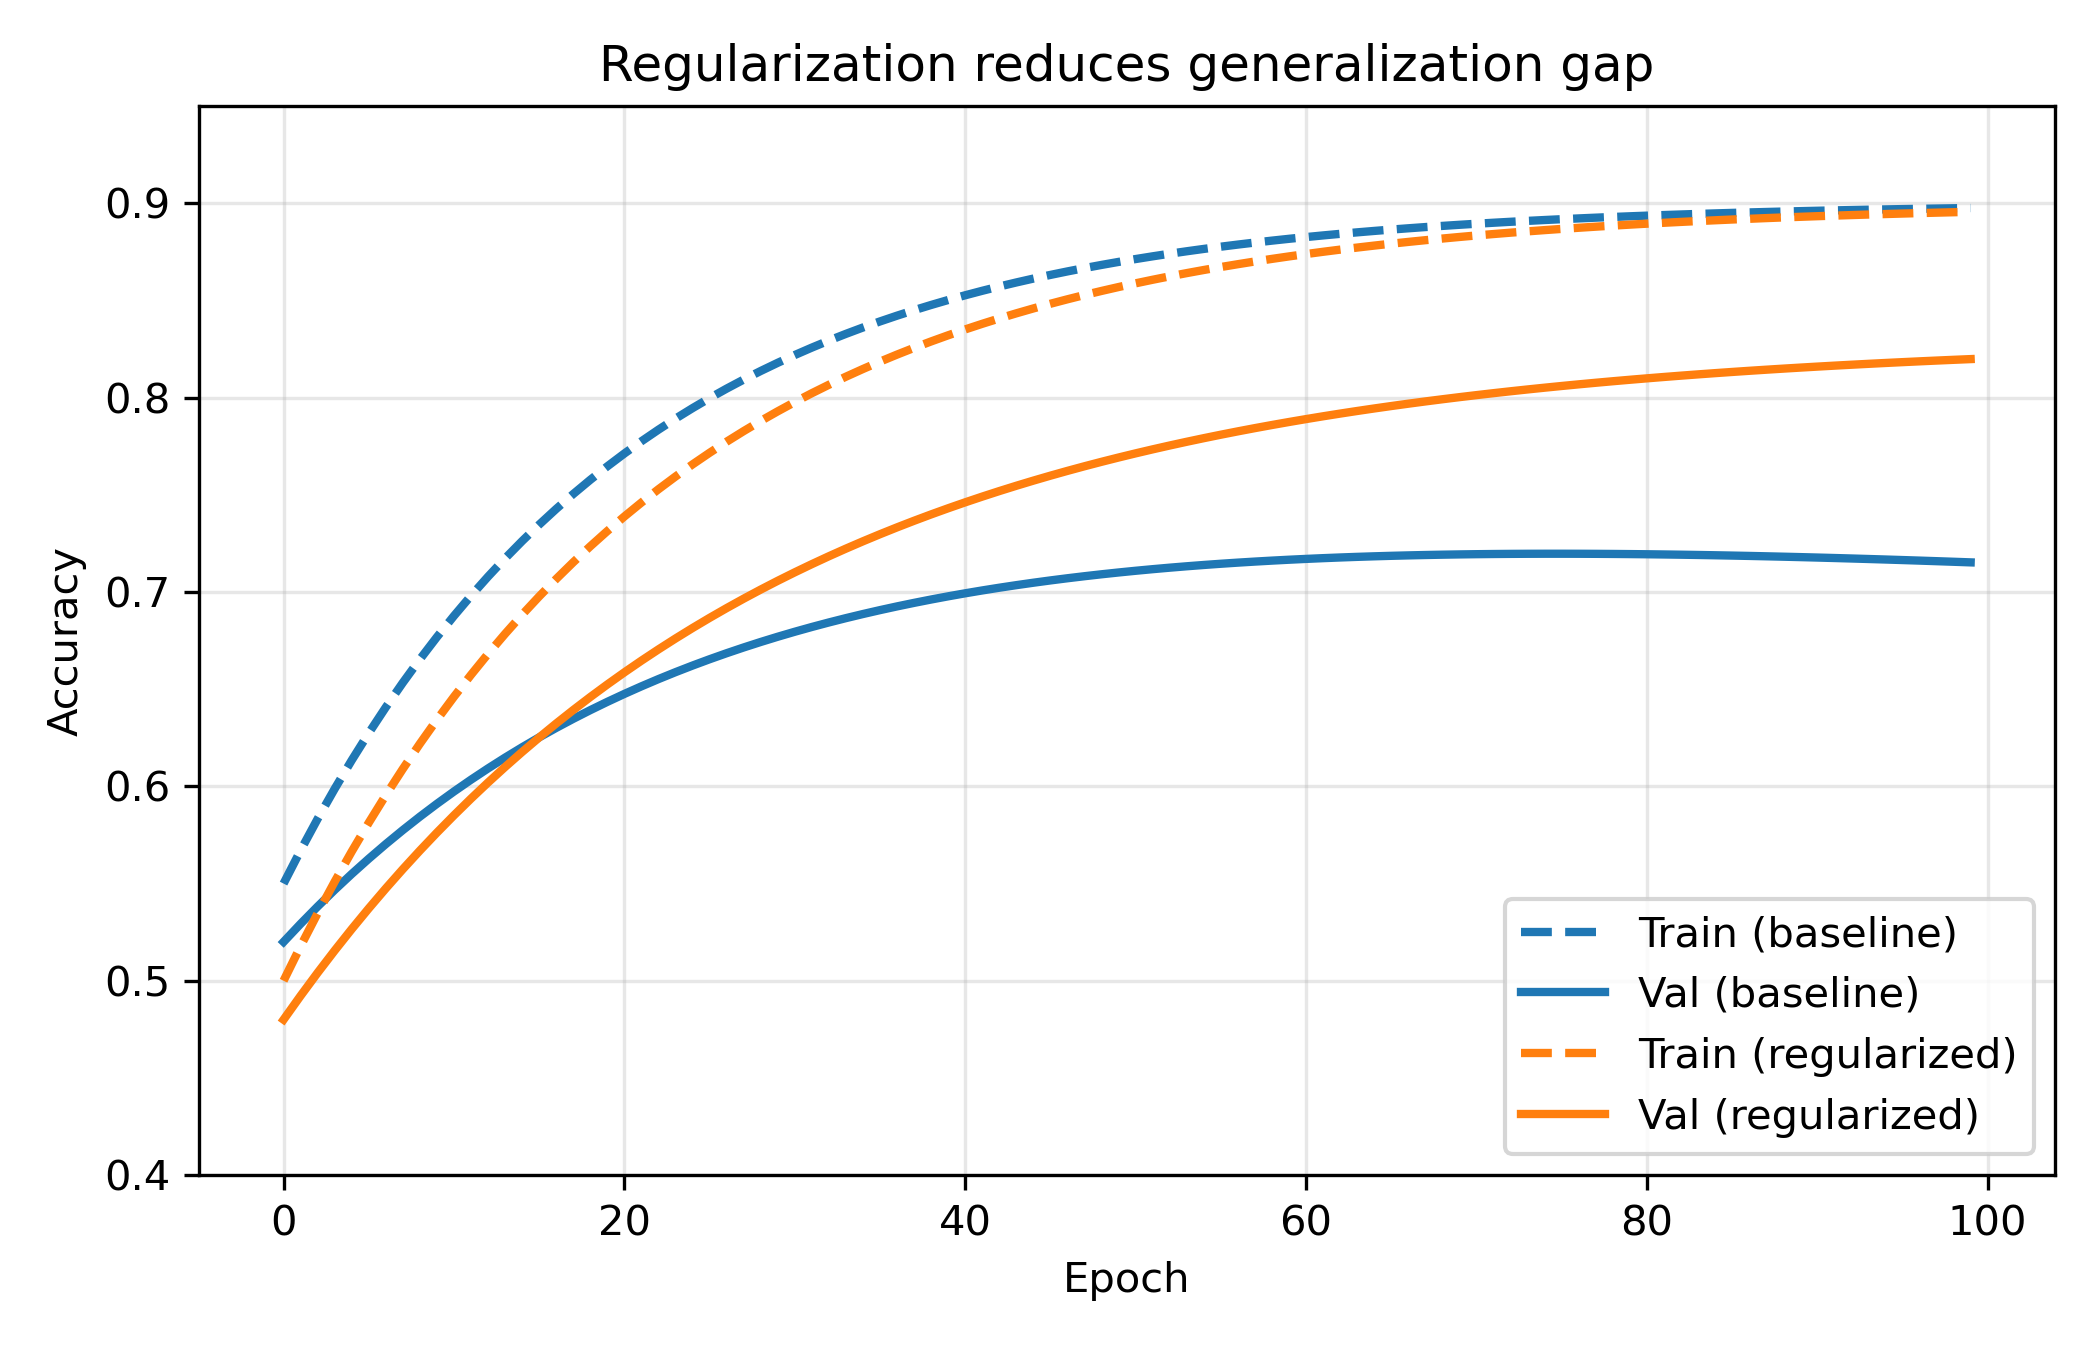
\includegraphics[width=0.8\linewidth]{regularization_effects.png}
  \caption{验证集准确率曲线展示正则化带来的泛化提升。}
  \label{fig:regularization_effects_cn}
\end{figure}
\FloatBarrier

\end{document}
